\section{Figures}
\label{apx:figures}

Images used in these figures fall under the Fair Use doctrine of U.S. Copyright law.

\begin{figure}[ht]
\caption{Rainbow Brain Usage}
\label{fig:brain}
\centering
  \subfloat[Rainbow Brain, as neurodiversity `cat paw' art.]{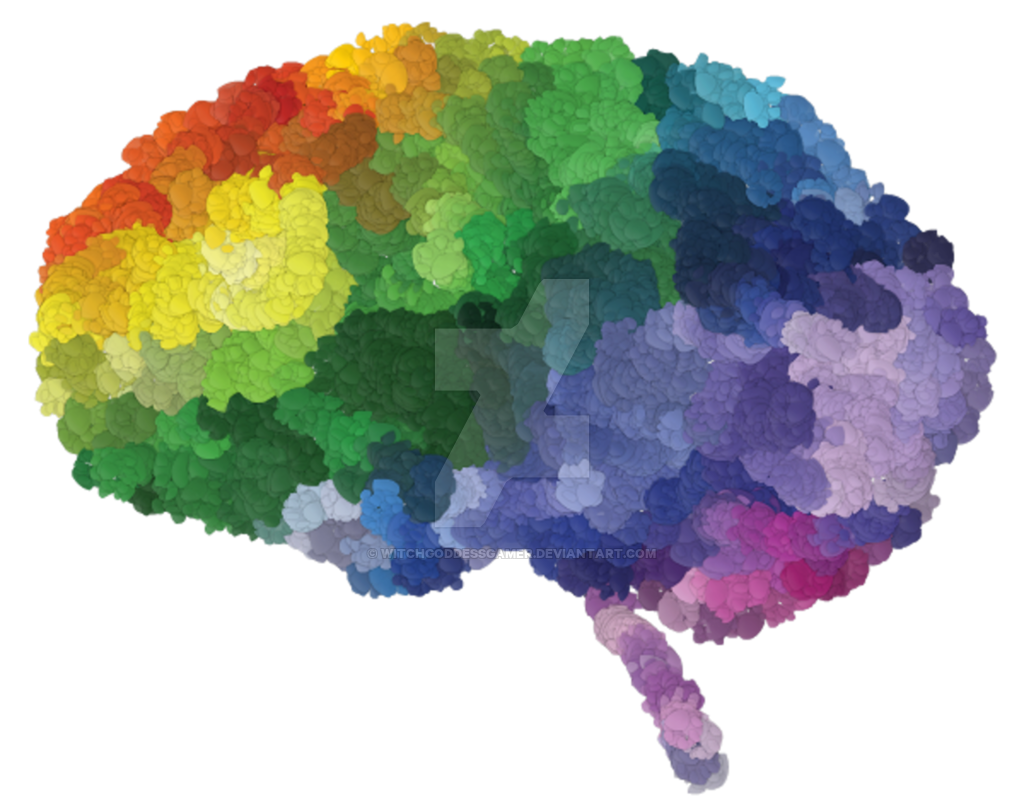
\includegraphics[width=0.3\textwidth]{cat_paw.png}}
  \quad
  \subfloat[Rainbow Brain, used as positive demographic identity on key badge.]{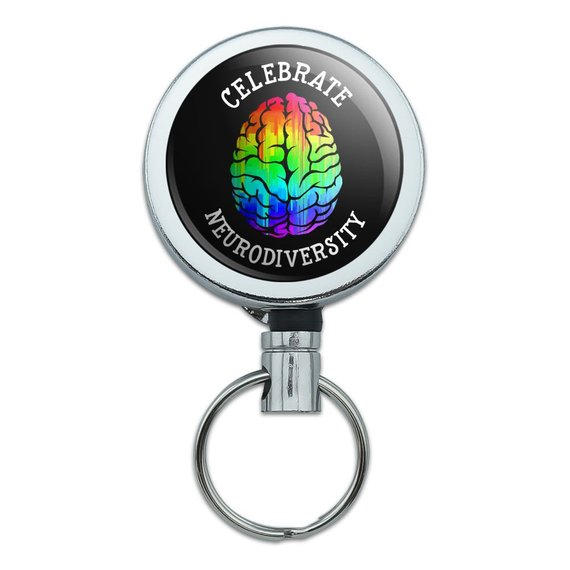
\includegraphics[width=0.3\textwidth]{keybadge.jpg}}
  \quad
  \subfloat[Rainbow arrangement of brains to celebrate neurodiversity.]{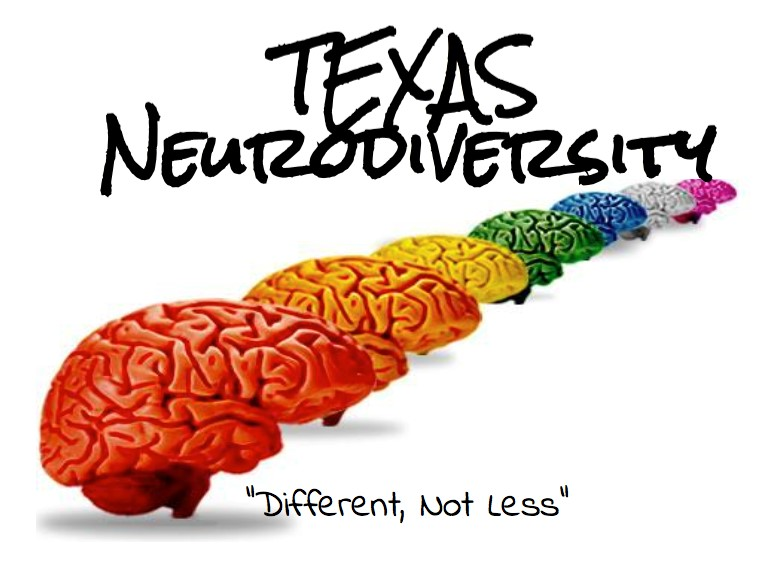
\includegraphics[width=0.3\textwidth]{texas.jpg}}
\end{figure}

\begin{figure}[ht]
\caption{Rainbow Infinity Loop Usage}
\label{fig:infinity}
\centering
  \subfloat[Rainbow Infinity Loop, used to encourage neurodiversity inclusion.]{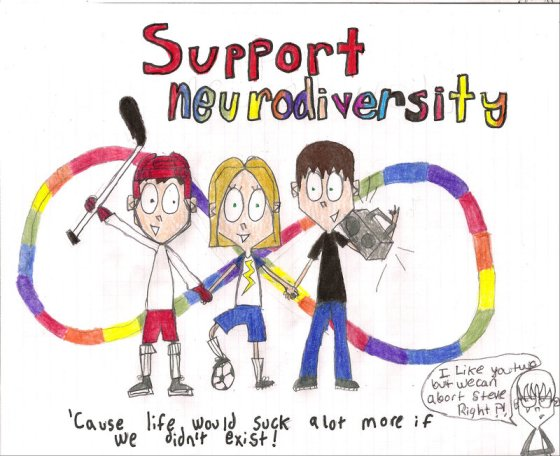
\includegraphics[width=0.3\textwidth]{infinity.jpg}}
  \quad
  \subfloat[Rainbow Infinity Loop Tattoo, used to express demographic identity.]{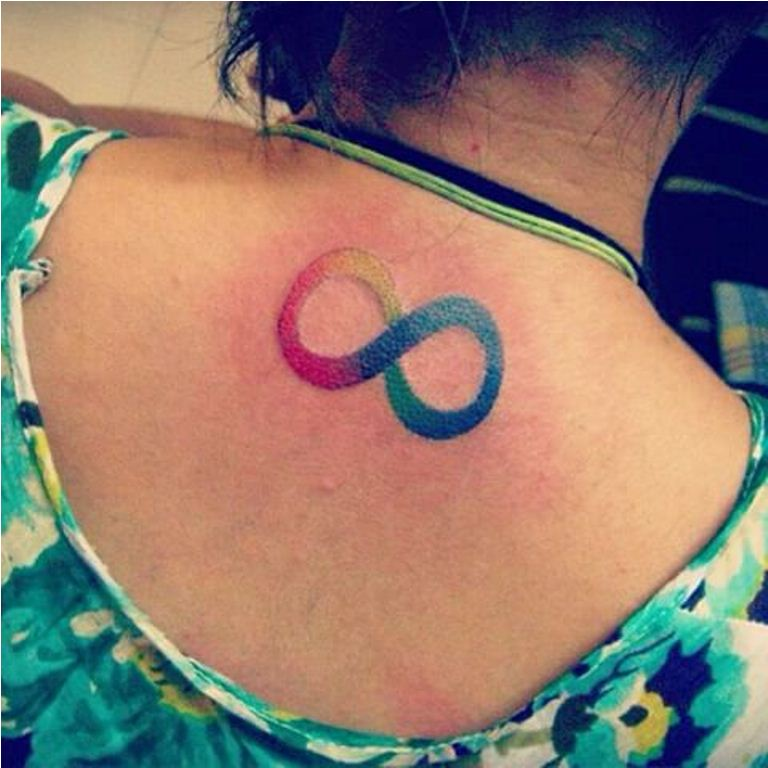
\includegraphics[width=0.3\textwidth]{20-rainbow-infinity-tattoo.jpg}}
  \quad
  \subfloat[Rainbow Infinity Loop, used as artwork for a Minecraft gaming platform mod.]{
\includegraphics[width=0.3\textwidth]{minecraft.png}}
\end{figure}

\begin{figure}[ht]
\caption{Autism Speaks Logo vs Twitter Emoji}
\label{fig:aspeaks}
\centering
  \subfloat[Autism Speaks Logo]{
\includegraphics[width=0.333\textwidth]{aspeaks}}
  \qquad
  \subfloat[Twitter Jigsaw Puzzle Piece Emoji]{
\includegraphics[width=0.25\textwidth]{twitterJigsaw}}
\end{figure}

\begin{figure}[ht]
\caption{Instructive Drawing of Brain using Multiple Colors}
\centering
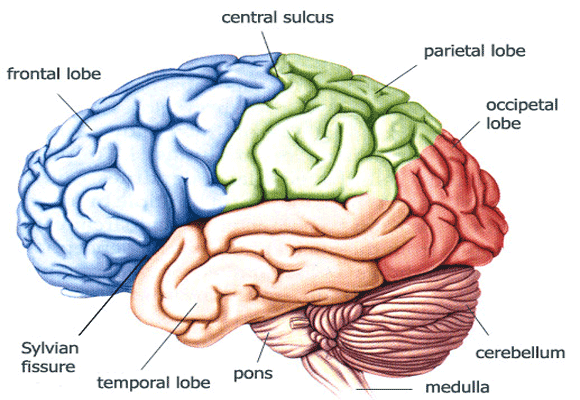
\includegraphics[width=0.5\textwidth]{brainparts.png}
\label{fig:brainparts}
\end{figure}

